\chapter{Techniques for Interactivity Support}
\label{chap:new_techiques}

%\todo{Where is the hotspot detection stuff?}

% simple dynamic bookmark placement and interactivity-aware content pre-fetching and replication

So far, this thesis has outlined a twelve month experiment in which highly interactive user behaviour was recorded. The traces obtained from the experiment have been analysed and characterised to produce a set of models and user workloads. These workloads and models were developed so future ideas and concepts could be designed and tested with realistic data.

This chapter outlines some of the improvements which can be made to aid in the delivery of this genre of content. This includes a system to dynamically position bookmarks within the media, a way to pre-fetch segments of the media ahead of their request, and an evaluation of hybrid delivery technique designed to deliver highly interactive content.

\section{Dynamic Placement of Bookmarks}
\label{sect:moving_bookmark}

During our experiments, bookmarks were appropriately positioned by administrators before the video was published. It was previously noted that a small percentage of bookmarks (roughly 6\%) were unintentionally misplaced. There are many reasons why a bookmark could be misplaced, such as human error, or a lack of insight into user requirements. For example: a bookmark could be placed before a penalty kick, but many users may first wish to see the foul that led to the penalty. As such, it would be beneficial if the system could autonomically detect poorly placed bookmarks and correct them based on automatic feedback derived from the user's actions.

During the second video trial, we took the opportunity to go beyond characterising user behaviour, by testing a dynamic bookmark placement technique in the live system. This technique inferred if the bookmark was misplaced based on the user's seeking behaviour, and then correct the bookmark's position in a reactive way. The remainder of this section discusses and analyse this technique.

%For example a football goal bookmark would be placed at the position the scoring team gained possession of the ball just before the goal. This allowed the user to view the run up to the goal, as well as the goal itself.


\begin{figure}[t]
    \centering

%    %http://www.ctan.org/tex-archive/graphics/pgf/doc/generic/pgf/version-for-pdftex/en/pgfmanual.pdf
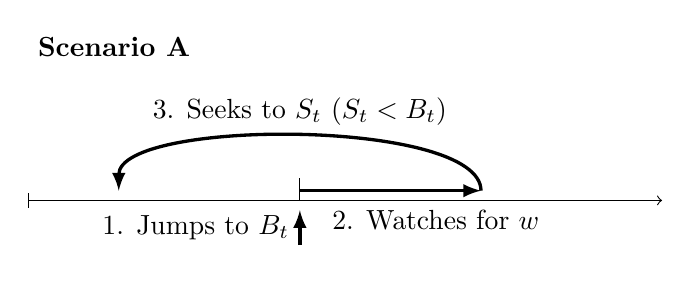
\begin{tikzpicture}[scale=2.3]

    \node[right] at (-1.5, 0.85) {\textbf{Scenario A}};

    \draw [|->] (-1.5,0) -- (2,0);
    \draw (0, 0) -- (0,0.125);

    \node (start) at (0,-0.3)  {};
    \node (bookmark) at (0,0)  {};
    \node (wait) at (1,0) {};
    \node (jump) at (-1,0) {};

    \begin{scope}[>=latex, very thick]
        \draw [->] (start.north) -- node[left] {1. Jumps to $B_{t}$} (bookmark.south);
        \draw [->] (bookmark.north) -- node[near end, below=3pt] {2. Watches for $w$} (wait.north);
        \draw [<-] (jump.north) .. controls +(up:0.4) and +(up:0.4) .. node[above] {
            3. Seeks to $S_{t}$ ($S_{t} < B_{t}$)
        } (wait.north);
    \end{scope}

    %\draw [|-|, dotted] (bookmark.south) -- node[below] {$d$} (jump.south);

\end{tikzpicture}

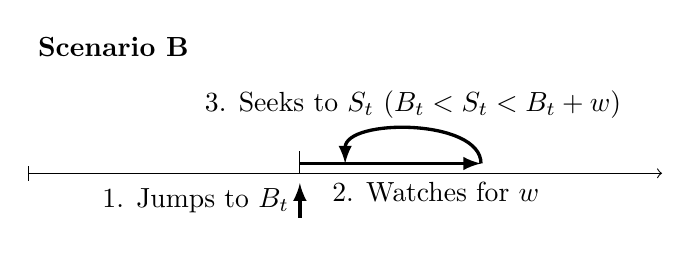
\begin{tikzpicture}[scale=2.3]

    \node[right] at (-1.5, 0.7) {\textbf{Scenario B}};

    \draw [|->] (-1.5,0) -- (2,0);
    \draw (0, 0) -- (0,0.125);

    \node (start) at (0,-0.3)  {};
    \node (bookmark) at (0,0)  {};
    \node (wait) at (1,0) {};
    \node (jump) at (0.25,0) {};

    \begin{scope}[>=latex, very thick]
        \draw [->] (start.north) -- node[left] {1. Jumps to $B_{t}$} (bookmark.south);
        \draw [->] (bookmark.north) -- node[near end, below=3pt] {2. Watches for $w$} (wait.north);
        \draw [<-] (jump.north) .. controls +(up:0.25) and +(up:0.25) .. node[above] {
            3. Seeks to $S_{t}$ ($B_{t} < S_{t} < B_{t} + w$)
        } (wait.north);
    \end{scope}

    %\draw [|-|, dotted] (bookmark.south) -- node[below] {$d$} (jump.south);

\end{tikzpicture}

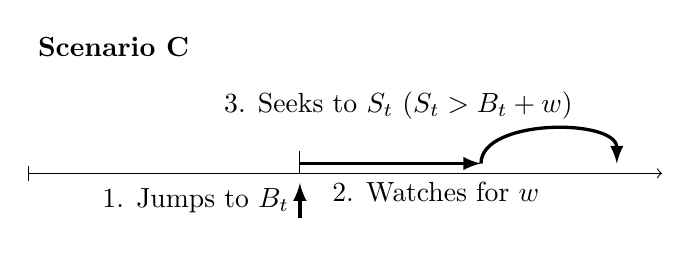
\begin{tikzpicture}[scale=2.3]

    \node[right] at (-1.5, 0.7) {\textbf{Scenario C}};

    \draw [|->] (-1.5,0) -- (2,0);
    \draw (0, 0) -- (0,0.125);

    \node (start) at (0,-0.3)  {};
    \node (bookmark) at (0,0)  {};
    \node (wait) at (1,0) {};
    \node (jump) at (1.75,0) {};

%TODO If have time maybe fix point 3 to be cantered better

    \begin{scope}[>=latex, very thick]
        \draw [->] (start.north) -- node[left] {1. Jumps to $B_{t}$} (bookmark.south);
        \draw [->] (bookmark.north) -- node[near end, below=3pt] {2. Watches for $w$} (wait.north);
        \draw [<-] (jump.north) .. controls +(up:0.25) and +(up:0.25) .. node[above left=12pt, pos=0] {
            3. Seeks to $S_{t}$ ($S_{t} > B_{t} + w$)
        } (wait.north);
    \end{scope}

    %\draw [|-|, dotted] (bookmark.south) -- node[below] {$d$} (jump.south);

\end{tikzpicture} 
    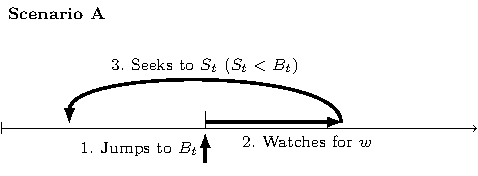
\includegraphics[width=0.7\columnwidth]{./diagrams/scenarios_A}
    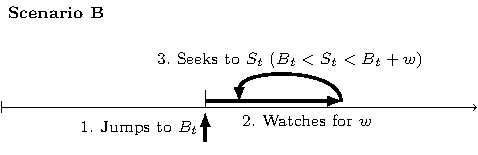
\includegraphics[width=0.7\columnwidth]{./diagrams/scenarios_B}
    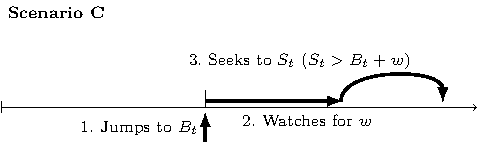
\includegraphics[width=0.7\columnwidth]{./diagrams/scenarios_C}

    \caption{Different scenarios that may induce bookmark movement}
    \label{fig:movingbookmark}
\end{figure}

To develop a reactive algorithm that moves bookmarks dependent on user behaviour, different possible scenarios should first be explained. \autoref{fig:movingbookmark} shows three different sequences of actions a user could follow shortly after seeking to a bookmark.

\begin{description}
  \item[Scenario A] shows the user briefly viewing the bookmark, then seeking to a time earlier than it. While this could indicate that the bookmarked event was short and that the user wanted to view it again, it could equally imply that the bookmark was placed later than it should have been.
  \item[Scenario B] is similar to \emph{Scenario A} but differs in that the user does not seek back to a point before the bookmark; this means the user is simply replaying footage, thus implying the bookmark is correctly placed for that individual.
  \item[Scenario C] represents a situation in which the user's motives are difficult to determine. Since they watch briefly then seek forward, several possibilities exist: the bookmarked event may have ended, the bookmark may have been placed prematurely, or the user is simply seeking forward towards the next event.
\end{description}

A further possibility, not shown in the figure, is for a user to seek far away from a bookmark in either direction. Since it is unlikely their destination would be related to the bookmark, such an action would not indicate the bookmark was incorrectly placed.

\emph{Scenario A} and \emph{Scenario C} are therefore the only scenarios where the user's actions could indicate the bookmark is misplaced. All other actions should reinforce the position of the bookmark to reduce future movements once it is correctly placed. Additionally since we are less sure of the user's intentions in \emph{Scenario C} we should only make minor changes to the bookmark's placement to limit the impact of false-positives.

\renewcommand{\algorithmiccomment}[1]{// #1}
\begin{algorithm}[t]
{\small
\begin{algorithmic}[0]
    \STATE\COMMENT{$B_{t}$ is the location of the bookmark at time $t$}
    \STATE\COMMENT{$S_{t}$ is the location the user sought at time $t$}
    \STATE\COMMENT{$w$ is the time the user waited before seeking to $S_{t}$}
    \IF {$S_{t} < B_{t}$}
        \STATE\COMMENT{\emph{The user seeks backwards before the bookmark}}
        \IF {$w <= 20$ \textbf{and} $S_{t} > (B_{t} - 60)$}
            \STATE\COMMENT{\emph{The seek occurred within 20 seconds of viewing the bookmark and lands within 60 seconds of the bookmark}}
            \STATE $\alpha = 0.1$
            \STATE $B_{t+1} = \alpha S_{t} + (1-\alpha) B_{t}$
        \ENDIF

    \ELSIF {$S_{t} > (B_{t} + w)$}
        \STATE\COMMENT{\emph{The user seeks forward}}
        \IF {$w <= 60$ \textbf{and} $S_{t} < (B_{t} + 120)$}
            \STATE\COMMENT{\emph{The seek occurred within 60 seconds of viewing the bookmark and lands within 120 seconds of the bookmark}}
            \STATE $\alpha = 0.05$
            \STATE $B_{t+1} = \alpha S_{t} + (1-\alpha) B_{t}$
        \ENDIF
    \ENDIF
\end{algorithmic}
}
\caption{Dynamic bookmark moving algorithm}
\label{alg:bookmark}
\end{algorithm}

\autoref{alg:bookmark} has been developed to identify these situations and act appropriately with regard to moving a bookmark. An exponential moving average (EMA) is used to recalculate the bookmark's position with a smoothing constant $\alpha$. The value used for $\alpha$ is dependent on the identified scenario. Initially these values were 0.1 and 0.05 allowing us to place greater confidence in the seeking-backward \emph{Scenario A} than the seeking-forward \emph{Scenario C}. These values were chosen as the intuitive first guesses for experimental purposes, and should be refined with future experiments. For our testing scenario we also used maximum wait times of 20 and 60 seconds for backward and forward seeks respectively. These maximum values were chosen because they exceeded approximately 80\% of all wait times.

%Note that 20s is used in the algorithm because 81.7\% of backward seeks were carried out in that interval, and 87.49\% of forward seeks within 60s}


\begin{figure*}[t]
    \centering

    \subfloat[][Position over time] {
        \label{fig:man-mil-time}
        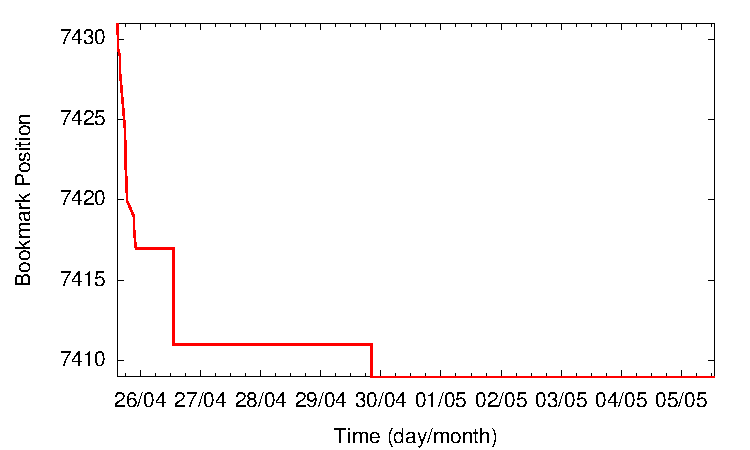
\includegraphics[width=0.5\columnwidth]{./graphs/mufc-mila_Goal_3-2_time}
    }
    \subfloat[][Position over requests for bookmarks] {
        \label{fig:man-mil-requests}
        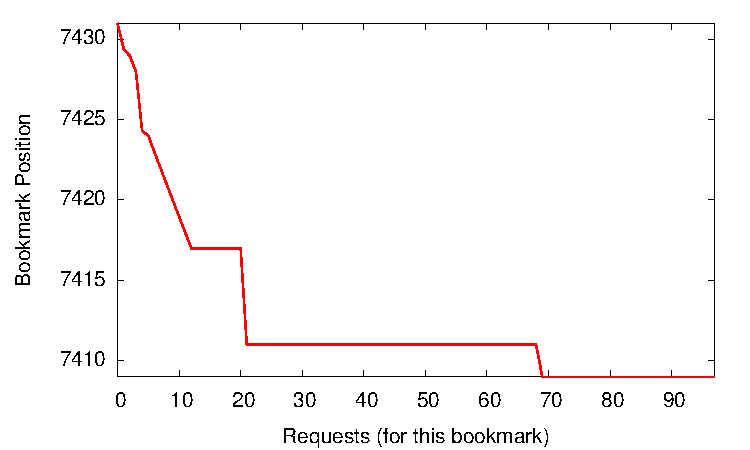
\includegraphics[width=0.5\columnwidth]{./graphs/mufc-mila_Goal_3-2_request}
    }

    \caption{Manchester United vs Milan single bookmark position}
    \label{fig:man-mil}
\end{figure*}

To test this algorithm, several of the bookmarks in the second video trial (not the initial World Cup experiment) were deliberately misplaced by different amounts before they appeared on the live site. Over time the bookmarks were moved autonomically by our algorithm. For example, \autoref{fig:man-mil-time} \& \autoref{fig:man-mil-requests} show the position of a single bookmark as it was moved by the system with respect to time and received requests. In both cases the system responds and the bookmark quickly moves to a new position, and then gradually converges until it becomes stable. In most cases the majority of movements were only in one direction, but for a couple of bookmarks the positions oscillated between two values. The most prominent example of this was a foul in a football match which led to a penalty. Some users wished to see the foul but others only wished to see the penalty a minute later. In these small number of cases it is subjective to decide if a bookmark is correctly placed, and in fact using this algorithm the bookmarks may never converge to a single point. In such cases, it may be best to bias the bookmark towards the earlier position, so both the early and later events can easily be seen.

\begin{figure*}[t]
    \centering

    \subfloat[][CDF of percentage reduction in viewing duration] {
        \label{fig:duration_saved_cdf}
        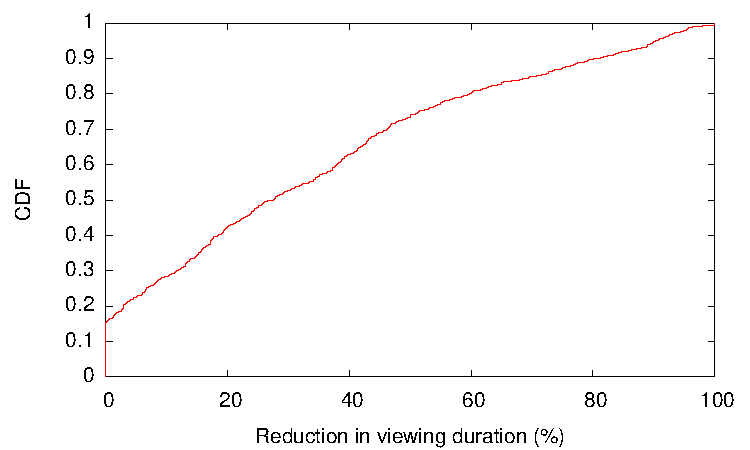
\includegraphics[width=0.5\columnwidth]{./graphs/moved_savedovertime_cdf}
    }
    \subfloat[][Percentage reduction in viewing duration versus received requests] {
        \label{fig:duration_saved_requests}
        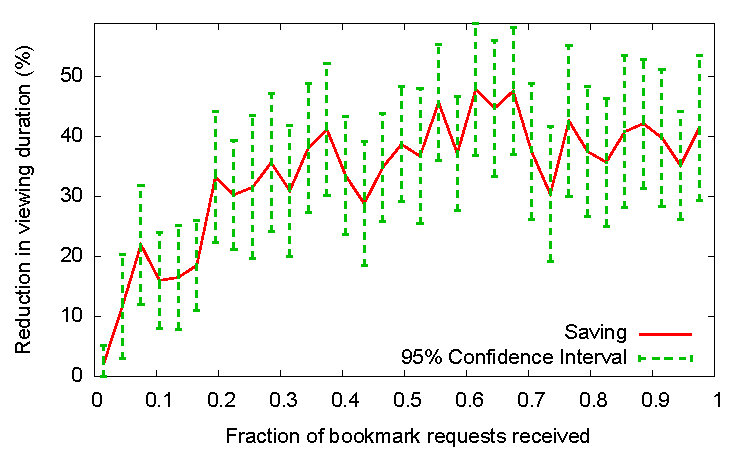
\includegraphics[width=0.5\columnwidth]{./graphs/moved_binned_savedovertime}
    }

    \caption{Reduction in viewing duration due to the algorithm}

\end{figure*}

%\todo{ Make reduction calc clearer }

Instead of subjectively deciding if a bookmark has moved to its correct location, we examined how much traffic might have been saved by moving the bookmark to a new location. If, for example, a bookmark was moved forward 10 seconds closer to the desired location, and a user views for 90 seconds, then by moving the bookmark we have potentially stopped video being transferred, which might have normally been skipped over. A reduction of $10/(90+10)=10\%$ is therefore made. Of course, this is only true if the user does not seek backward to watch the skipped 10 seconds, in which case we save nothing, and in fact incur an extra seek. \autoref{fig:duration_saved_cdf} displays a CDF of the potential reduction in viewing duration per bookmark request from the use of the algorithm. We can see that 16\% of the requests made no saving: these are accounted for by early requests before the bookmarks were moved, and requests where the user incurs an additional seek.

%seeks between the original and current bookmark location. %The remaining 84\% of request reduced the play

\autoref{fig:duration_saved_requests} illustrates how rapidly these reductions are made (and whether or not they are sustained) through a plot of the fractional potential saving versus the number of requests received across all the moved bookmarks. For the first 20\% of requests the reductions are low yet they improve, and then stabilise at a reduction of between 30-40\% per request. The 95\% confidence intervals are quite wide in most cases (averaging around $\pm$10 seconds) although this variance is mostly due to differences in playback length and not the 16\% of requests with no saving.

With minimal processing this simple algorithm has been able to reposition the bookmarks to more appropriate locations based on observed user behaviour, resulting in consistent traffic reductions. The algorithm can still be improved by fine tuning the $\alpha$ values. Larger values would move the bookmark more quickly at the cost of increasing the probability of incorrect decisions. This investigation has been left for future work.

%\begin{figure}[t]
%    \centering
%    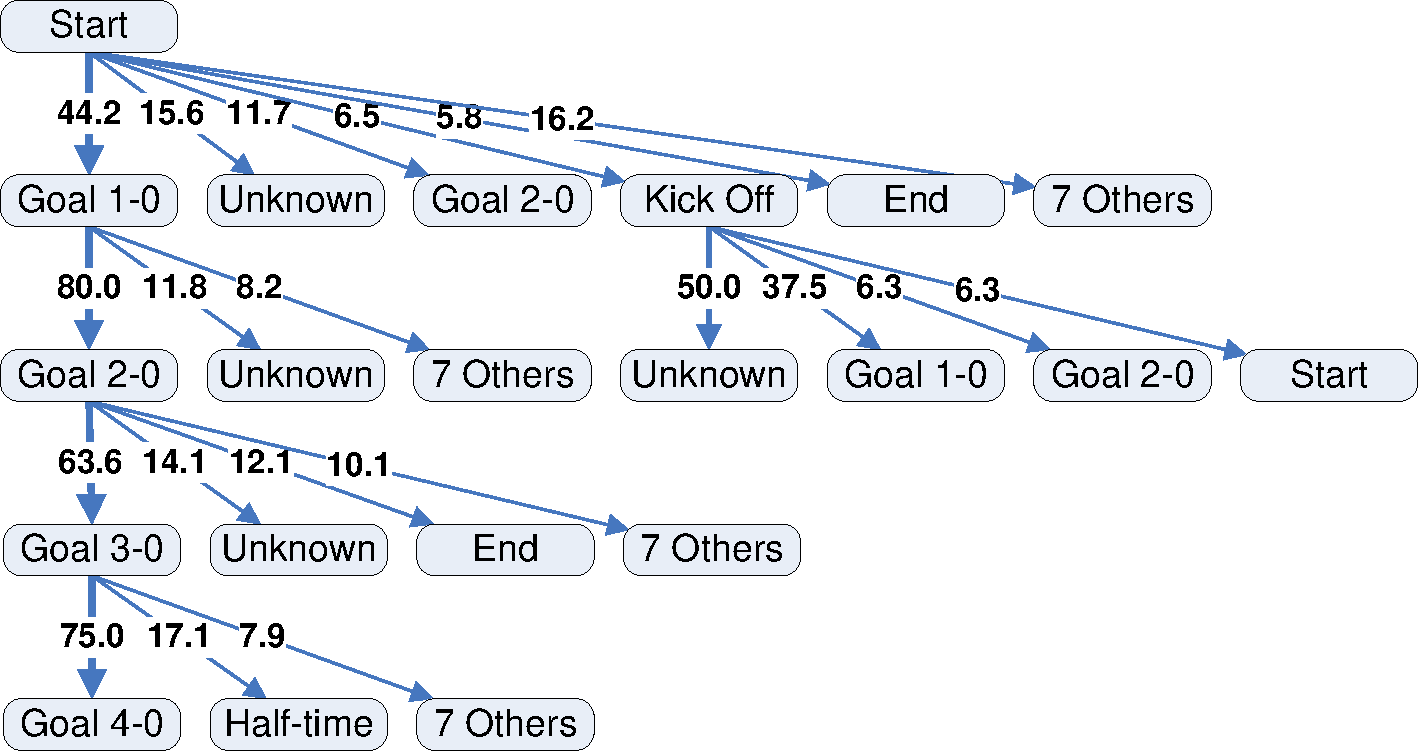
\includegraphics[width=0.5\textwidth]{./diagrams/sequence.png}
%
%    \caption{Graph of the order bookmarks are clicked. Note: This is a work in progress, and doesn't display well so I'll send links around to larger pngs.}
%%    \label{fig:mil-man}
%\end{figure}

%   Before  After   Distance            Best
%mufc-mila_Goal 1-2 3185    3168    17  Late            *interesting, because bookmark was well placed (but got moved)
%mufc-mila_Goal 3-2 7431    7409    22  Late        7417.808
%liv-che_Goal 1-0   2286.185    2187    99.185  Late
%ita-fra_Penalty 1-0    3915.718    3904    11.718  Late
%mil-man_Goal 3-0   8433.083    8415    18.083  Late
%mil-man_Goal 2-0   4505    4473    32  Late
%mil-man_Goal 1-0   3260    3277    -17 Early       3299.81

%notes
%Rates of seeks over time
%Find the end of bookmark
%change the sequence graphs (to show direction, correct weights), and possible add another "didn't jump" state
%what time do they jump out?

% How many times was a segment re-watched, and how soon between watching? Indicates how useful local buffering old content would help

%\autoref{fig:man-mil} show the position of a single bookmark in the Manchester United vs Milan over time. This bookmark was purposely placed too late by 15 seconds, causing frustrated users to rewind. \autoref{fig:mil-man} shows the placement of a Milan vs Manchester United bookmark which was placed 30 seconds too early.


\section{Predictive Pre-fetching}

In the classic start-to-finish model it is commonplace to simply pre-fetch ahead of the playback point. This reduces the chance of playback stalling due to momentary network problems. However, due to the increased interactivity of users and their departure from the start-to-finish model, it is no longer wise to only pre-fetch ahead of the playback point. As noted in \autoref{sect:sequence} it is possible to predict which bookmark a user will view next, allowing the client to intelligently pre-fetch content, benefitting both clients and servers.

For the clients, pre-fetching removes seek latency when seeking to a pre-fetched segment, both in terms of incurred network seek latency and also the time taken to buffer enough video for playback.  Pre-fetching also helps to avoid buffer underruns under poor network conditions. Similarly, on the server side, pre-fetching can help reduce the peak server load by increasing the load at quieter times with pre-fetching requests, thus making the overall load more uniform.

%Figure~\ref{fig:server_load_a} gives an example of server load at different times. The shaded areas show the server going over some limit, perhaps the server's bandwidth capacity. If pre-fetching is used this load could happen earlier whist staying below the server's limit as shown in Figure~\ref{fig:server_load_b}.

However, pre-fetching does come with a cost; resources are wasted if a segment is downloaded and never used. Deciding which segments to pre-fetch is therefore an important task. This section gives some background on the concept of pre-fetching, followed by the design and evaluation of a pre-fetching technique for our highly interactive workloads.

\subsection{Background}
    %Nic has read

    % TODO, maybe try and incorporate the following
    %"Exploring prefetching to improve the scalability of these protocols for interactive workloads is left for future work."~\cite{costa2004aci}

    % Many forms of pre-fetching
        % Pre-fetching (or Pre-loading) videos before you even request them
        % Buffering ahead of the current playback point
        % Pre-fetching segments within the video
    % Pre-fetched data may be pulled to a local STB, or a local cache server~\cite{sen99ppc,eager1999orc}
    % Pre-fetched data may be fetched from broadcast streams, server, or other nodes

    Pre-fetching or pre-loading, is the act of requesting content in advance of demand. This allows clients to have the requested media stored locally before needing it. When a client eventually does request the media, it can be served from the local cache, as opposed to requesting it from a server. Pre-fetching can therefore improve the experience for clients, as there is reduced start-up delay, at the cost of pre-fetching content which may never be viewed.

    %Servers can also benefit from pre-fetching, for example, if the content is pre-fetched when the server has spare capacity, it will hopefully reduce load at peak times.

    There are a three main forms of pre-fetching. The first is pre-fetching the media before playback. The second is when playing media, to buffer slightly ahead of the playback point. The last is to pre-fetch segments of media while the media is being played. These three forms will now be discussed in more detail.

    When the media is fetched before playback has began it is typically called pre-loading. This involves either fetching the full media, or just the beginning segments of the media~\cite{paris2001cap}. Pre-loading the beginning segments is typically used to reduce the start-up latency when the media is periodically broadcast~\cite{paris1999zdb}. The decision of what to pre-load is normally based on what content is popular, and how much spare capacity the server has. There have been numerous papers detailing the optimal parameters~\cite{barnoy2008odm}, such as how much to pre-fetch~\cite{paris2001stp}, how many objects to pre-fetch~\cite{paris2002bpv}, how much bandwidth to use, what delivery mechanism to use~\cite{chung2003evb}, \emph{etc}. From the work, it seems clear that the exact parameters are dependant on the characteristics of the media, as well as how the media is delivered. But overall, pre-fetching at least the first few minutes of media certainly provides benefits.

    A very common pre-fetching technique is to buffer ahead of the playback point. This requires a small buffer, large enough to contain at least a few seconds of media. Before playback begins, this buffer is filled and then playback may start from the buffer. The buffer smooths out playback, allowing it to be jitter free, as well as hiding temporary network problems, such as lost packets. This kind of pre-fetching is also useful when streaming variable bitrate (VBR) content~\cite{reisslein1997jsq}. Typically, VBR content is bursty, causing periods of time where the server is either under-utilised or oppositely, unable to satisfy the demands of its clients. To solve this, each client requests the VBR content at a constant bitrate (equalling the mean VBR rate), allowing the client's local buffer to smooth out the burstiness~\cite{bakiras1999sap}.

    The final technique is to pre-fetch segments which are likely to be viewed within the content. This is one of the main areas of interest in this section. The pre-fetched segments can be areas within the media which are particularly popular, and are likely to be watched. Popular segments may occur when users selectively seek within the media and do not follow the typical start-to-finish model of playback. As far as this author is aware, there has been no work which will pre-fetch segments of media in this manner.

    The closest example of such pre-fetching, is ``link pre-fetching'' used by some web browsers and proxies~\cite{chinen1997ipp}. This feature will pre-fetch hyperlinks on the web page that the user is currently viewing. In this way, if the user clicks on a hyperlink which has been pre-fetched, the page will load instantly. However, this technique has been discouraged~\cite{davison2001apg}, as most of these systems blindly fetch all hyperlinks on the page. This generates additional bandwidth, and may overload the servers~\cite{duchamp1999ph}.

    When content is pre-fetched, it is not always stored in the same place. Earlier work assumed that pre-fetched content would be stored on content servers near to the clients~\cite{sen99ppc,eager1999orc}. More recent work has assumed that clients are using a set-top box (STB) or PC to view the media, both of which may contain a large hard disk or similar storage device. This allows the content to be available even when the client has no connectivity.

    Pre-fetching does not always have to involve a server. In the most na\"{i}ve systems, pre-fetched data is requested directly from the server via unicast distribution. More advanced systems have dedicated pre-fetch channels which periodically broadcast the segments of media which the server deems useful to pre-fetch~\cite{chung2003evb}. More recently, systems have been designed to pre-fetch media from neighbouring clients~\cite{shen2006dps}. One study by Huang~\emph{et~al.} found that if peers used their spare upload to assist others in pre-fetching, the server's bandwidth could be significantly reduced~\cite{huang2007civ}.

\subsection{Pre-fetching Strategies}

The workloads observed in this thesis exhibited sparsely distributed areas of high interest. This areas have been dubbed ``hotspots''. A sensible pre-fetching strategies would take advantage of these hotspots, and pre-fetch their segments accordingly.

Therefore, a set of pre-fetching strategies were devised. For simplicity, and because interest typical formed around bookmarks, each strategy will only pre-fetch segments immediately following a bookmark (\emph{i.e.}, bookmarked hotspots). In all experiments the amount of each hotspot pre-fetched was determined by varying the percentile of that particular hotspot's length model, as described in \autoref{sect:hotspot_length}.

Each pre-fetch strategies was tested within a simulator driven by the \emph{eurovision} trace. Clients were provisioned with a dedicated link to the server, capable of transferring twice the bitrate required to play the content. Once a client has fetched enough data to fill a 5 second playback buffer, half of their bandwidth is allocated to the pre-fetcher whilst the other half continues to fill the playback buffer.

The details for each pre-fetch strategy are listed below:

%Simulations were run using real \emph{eurovision} traces obtained from our system to test these different strategies. \emph{Eurovision} was chosen due to its popularity and  representative nature. As soon as the client starts playback of a video a separate thread begins to pre-fetch segments (at playback rate) which the scheme anticipates the client will need. Connections between the clients and server were highly provisioned and never congested. In all experiments the amount pre-fetched for each bookmark was determined by varying the percentile of that particular bookmark's length model, as described in Section~\ref{sect:hotspot_length}.

%We used different pre-fetching strategies, each using different information to decide which segment to fetch next. For simplicity, and because interest always formed around bookmarks, each strategy will only pre-fetch segments immediately following a bookmark (bookmark hotspots). %Hotspots always focused around bookmarks therefore these were a good choice to prefetch. However the length of these hotspots were not always know, so as you will see later, arbitrary values were used for the length of the pre-fetched segment.
%The different pre-fetching strategies tested are explained as follows:

%    \textbf{Before Start} pre-fetches all the bookmark hotspots before the user begins any playback. This demonstrates how well pre-fetching everything in advance will perform.

%    \textbf{Best} uses knowledge of future events to pre-fetch the bookmark hotspot that the user is actually going to view next. This is impossible to implement in practice, so this technique is for reference only. %Similar to Belady's minimum.

\begin{description}
  \item[Ahead] simply continues to pre-fetch ahead of the playback point assuming the client has a unlimited buffer. This is similar to what most existing streaming applications do.

  \item[Ahead (to hotspot end)] again simply continues to pre-fetch ahead of the playback point but only until the end of hotspot associated with the bookmark being viewed.

  \item[Ahead (and Predictive)] works in a similar way to \emph{Ahead (to hotspot end)}, however, once it reaches the end of the hotspot it begins to use the \emph{Predictive} pre-fetch scheme.

  \item[Predictive] uses knowledge observed from other users as to which bookmark is likely to be requested next, and thus starts to pre-fetch the bookmark hotspots in descending order of probability of being visited. This uses the sequence tree concept introduced in \autoref{sect:sequence}, therefore the more users interacting with the system, the more accurate the predictions becomes.

  \item[Sequence] will pre-fetch bookmark hotspots in the order in which they appear within the video regardless of the current playback point. For example, in a football match the bookmarked goals would be pre-fetched in a sequential order.

  \item[Sequence After] again pre-fetches bookmark hotspots in the order in which they appear within the video; the difference being only hotspots that are after the current playback point are fetched. For example, if a user has yet to fetch the first bookmark's hotspot but is already viewing the second, then the first will not be pre-fetched.

%  \item[Random] will pre-fetch the bookmark hotspots in a random order.
%  \item[Popularity] pre-fetches the bookmark hotspots in order of their overall popularity.

\end{description}


%Simulations were run using real \emph{eurovision} traces obtained from our system to test these different strategies. \emph{Eurovision} was chosen due to its popularity and  representative nature. As soon as the client starts playback of a video a separate thread begins to pre-fetch segments (at playback rate) which the scheme anticipates the client will need. Connections between the clients and server were highly provisioned and never congested.

\begin{figure*}[t]
    \centering

    \subfloat[][Fraction of requests with zero seek latency] {
        \label{fig:eurovision_instaseek}
        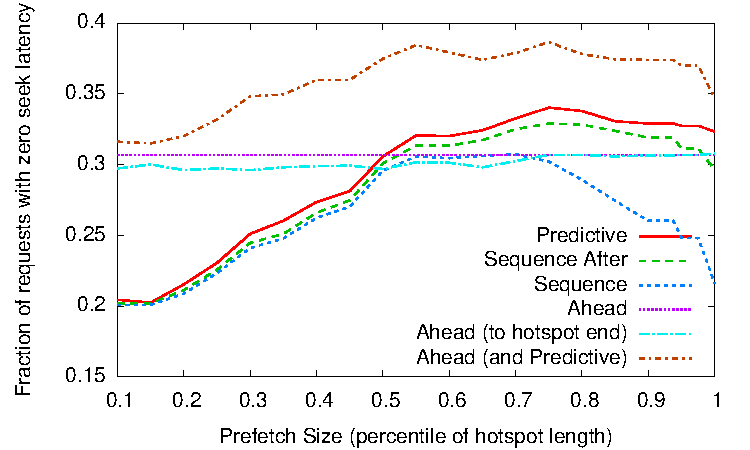
\includegraphics[width=0.5\columnwidth]{./graphs/1206722178-eurovision_tab-instaseek}
    }
    \subfloat[][Usage ratio] {
        \label{fig:eurovision_usage}
        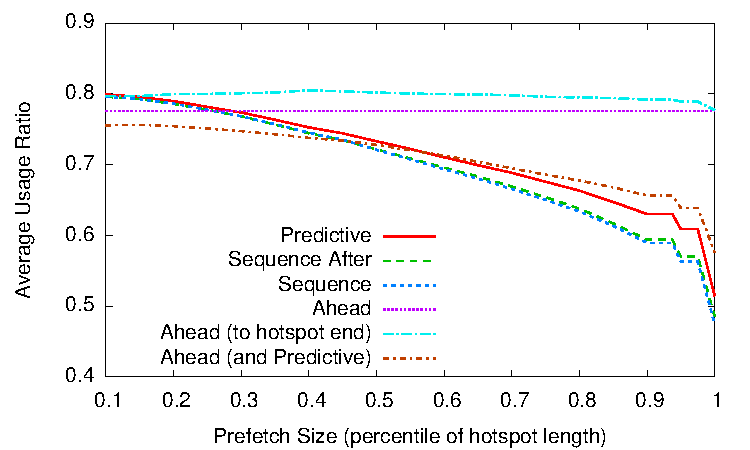
\includegraphics[width=0.5\columnwidth]{./graphs/1206722178-eurovision_tab-usage}
    }

    \caption{Various metrics for different pre-fetch schemes versus bookmark length}

\end{figure*}

Two metrics were measured to determine how well the different schemes behaved. The first metric displayed in \autoref{fig:eurovision_instaseek} is the fraction of requests with zero seek latency. A seek latency of zero occurs when the user has already pre-fetched a playback buffer's worth of video from a requested seek point. The second metric measured the ratio of fetched data which was never watched, and therefore needlessly fetched. This usage ratio is shown in \autoref{fig:eurovision_usage}.

Using the simple \emph{Ahead} scheme 31\% of seeks have zero latency, this is made up of seeks to segments that have already been viewed, and small forward seeks into the ahead buffer. Adapting this scheme to only pre-fetch to the end of the bookmarks (\emph{i.e.} the \emph{Ahead (to hotspot end)} scheme) has a minor negative effect on the seek latency, whilst increasing the average usage ratio.

The \emph{Sequence} and \emph{Sequence After} schemes are very similar, but the simple modification to the \emph{Sequence After} scheme allowed it to achieve a lower seek latency whilst not degrading its average usage ratio. This was because users had a tendency to not seek to a bookmark before the current playback point, and always go forward within the video, leaving the \emph{Sequence} scheme stuck pre-fetching hotspots before the current playback point.

Both the \emph{Predictive} and the \emph{Sequence After} schemes perform in a similar manner, with the \emph{Predictive} schemes always outperforming the other. Due to this fact, the \emph{Sequence After} scheme could be used in place of the \emph{Predictive} scheme whilst knowledge is collected to improve the \emph{Predictive} scheme's accuracy.

The best outcome was the combination of \emph{Ahead} and \emph{Predictive} schemes named \emph{Ahead (and Predictive)}. This exploited the fact that users rarely viewed beyond the end of a hotspot, and thus pre-fetching another hotspot was of benefit.



%This has left unanswered however if pre-fetching segments based on the beginning of the bookmark is the best solution, whereas pre-fetching smaller grained segments might be better.
%So far these results look promising, however there is room for improvement.

%As expected, the \emph{Before Start} and \emph{Best} schemes outperformed all others. The \emph{Predictive} and \emph{Sequence After} schemes both performed equally catching at most 23\% of seeks, and the \emph{Popularity}, \emph{Sequence} and \emph{Random} schemes also performed equally albeit roughly 5\% lower than the \emph{Predictive} and \emph{Sequence After} schemes.
%It is interesting to note that using the popularity of the bookmark is not as effective as using the somewhat na\"{\i}ve \emph{Sequence} scheme. This is because while the \emph{Popularity} scheme is pre-fetching the most popular bookmarks (which could be towards the end of the video), the \emph{Sequence} scheme is fetching closer bookmarks which will be used sooner.
%As the pre-fetch size becomes larger most schemes are able to offer more zero latency seeks due to aiding seeks that occur shortly after the bookmark (\emph{e.g.}, seeking 15 seconds forward). However the improvements begin to diminish around 60\% as excess data is pre-fetched and thus time would be better spent fetching a different bookmark.

%Each scheme may pre-fetch different amounts of data. For example, the \emph{Best} scheme will keep trying to pre-fetch the bookmark hotspot that the user will view next, but if there is no following bookmark the scheme stops pre-fetching. Figure~\ref{fig:eurovision_usage} displays the amount pre-fetched data that was actually used for playback. The \emph{Best} scheme performs at least twice as well as any other listed, with the \emph{Before Start} performing worse since it has pre-fetched far more data than actually gets used. From the remaining schemes, \emph{Predictive} is consistently the best, achieving between 31\% and 39\% usage.
%
%Finally, we observe the overall byte hit/miss ratio in Figure~\ref{fig:eurovision_ratio}. This is how many bytes were successfully served by pre-fetched data versus the total number of bytes requested. Again, the different schemes performed similarly, with \emph{Predictive}, \emph{Sequence After}, and \emph{Popularity} performing equally. However, none of the schemes, including \emph{Before Start} achieved a satisfactory hit-ratio. At best, the realistic schemes achieved less than 20\%. This may be because the bookmark hotspots do not sufficiently cover the area requested by the users. Future work could therefore incorporate strategies that pre-fetch more than just hotspots following a bookmark.
%
%From these results it is clear the \emph{Predictive} and \emph{Sequence After} schemes perform best, with the \emph{Predictive} scheme slightly outperforming \emph{Sequence After} by having a higher pre-fetched utilisation. One aspect that has not been investigated is how quickly reliable knowledge needed for the \emph{Predictive} scheme can be obtained through other users' interactions. As such, a hybrid approach could be taken, beginning by using the simple yet effective \emph{Sequence After} scheme, switching to the \emph{Predictive} scheme once sufficient statistics have been acquired.
%
%The \emph{Best} scheme outperformed all others which suggests room for improvement in the other pre-fetching algorithms. The results presented are, however, perhaps the worst case since each client is working independently. If the clients collaborated, a shared pre-fetching network cache could result, thus increasing the hit/miss ratios while decreasing the load on the CDN.

\subsection{Pre-fetching Knowledge}

\begin{figure}[t]
    \centering

    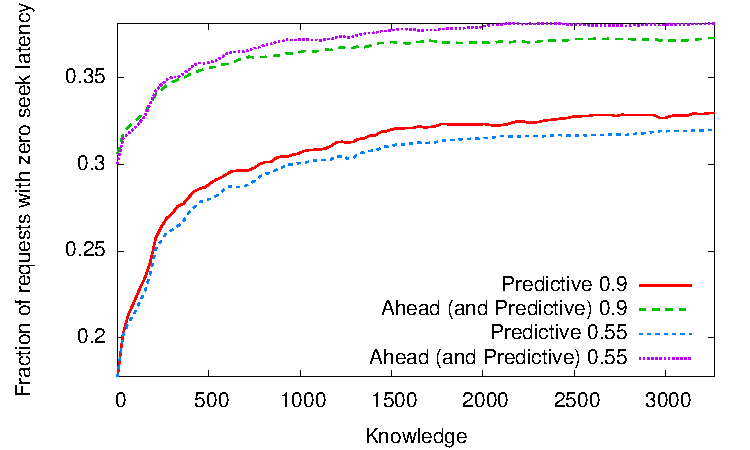
\includegraphics[width=0.5\columnwidth]{./graphs/1206982048-eurovision_tab_average-seek-knowledge}

    \caption{How zero seek latencies is effected by amount of pre-fetch knowledge}
    \label{fig:eurovision_knowledge}

\end{figure}

In the previous experiments the \emph{Predictive} scheme was primed with knowledge from all users, but in reality this knowledge would be built up over time. To test how quickly this knowledge could be obtained, we ran another set of experiments where the \emph{Predictive} and \emph{Ahead (and Predictive)} schemes were primed with different amounts of knowledge. The results of this are shown in \autoref{fig:eurovision_knowledge}. We set the percentile hotspot length to 0.55 and 0.9, which were chosen since 0.55 is where the seek latency began to stabilise, and 0.9 is where the usage ratio began to drop rapidly. The knowledge is ranked from 0 to 3000 which represents the number of seek requests the knowledge was based on. It can be seen that very quickly (within 250 seek requests) the knowledge has become useful, and eventually plateaus at 1500 seek requests. Any seek requests after this point just increase the confidence in the knowledge and does not improve it.

\begin{table}[tb]
\centering {
    \begin{tabular}{|cccc|}
      \hline
\setrowcolor{TableRowHead}
      Media & From (seconds) & To (seconds) & Frequency \\
      \hline
\setrowcolor{TableRowA}
      arg-scg  & 0    & 1024 & 34 \\
\setrowcolor{TableRowB}
      arg-scg  & 0    & 271  & 10 \\
\setrowcolor{TableRowA}
      arg-scg  & 0    & 0    & 5 \\
\setrowcolor{TableRowB}
      arg-scg  & 271  & 1024 & 8 \\
\setrowcolor{TableRowA}
      arg-scg  & 279  & 1024 & 2 \\
      \hline
    \end{tabular}
} \caption{Example links table, showing the frequency of seeks from one time to another}
\label{tab:links}
\end{table}

In a real system, predictive knowledge must be collected in real time, and then disseminated in an efficient, scalable, and quick way otherwise any benefits gained may be lost in overheads. One solution to gathering this knowledge is described below.

% Nic prove read on 9th Sept (all but last 2 paragraphs)

To gather this knowledge, the clients and servers must store a small amount of state. Clients must record what is currently being requested. These details are typically recorded by the client anyway, for example, the name of the media, as well as the location playback started within the media. To make the solution scale, and generate less overhead for the server, it has purposely been designed so that the server need not store per-client state. The servers must only store a table of links relevant to the media stored on that server.

An example of the server's links table is shown in \autoref{tab:links}. This table maps the frequency of seeks between two locations within the media. For example, \autoref{tab:links} shows that 34 seeks occurred between time 0, and time 1024 within the \emph{arg-scg} media. This table may be used by the server or clients to predict what they will visit next, for example, if a user has just started playback of \emph{arg-scg}, they have a $34/(34+10+5)$ or 69\% probability of seeking to time 1024 within the media.

To construct this table the client must send some additional information to the servers. Typically when a client seeks, a new request is issued and the old request is stopped. This new request may be issued to a different server if the media is partitioned across multiple servers, or just for load balancing purposes. So when a client issues a new request, it must send details of the new seek location to the previous server. These details can be sent when the client stops the previous request.

By sending details of the new request, the previous server is able to infer a link between the two requests, even if the next request is supplied by a different server. The server does not need to store any additional per-client state, at the cost of trusting that the client will always send correct information. The inferred links can be stored in a table along with the frequency of their occurrences. This is the beginning of constructing a prediction tree. Once sufficient links have been inferred, a tree can be constructed.

Once this links table begins to be constructed, it can be used by both the servers and clients. When a user makes a request, the server can send a subset of the table to the client as out-of-band data. For example, if the client requests second 0, then the server would send the subset of rows whose \emph{from} time is 0. This would give the client the knowledge to predict which locations are most likely to be visited following the current location. As the client continues playback, the server can send additional subsets of the table. For example, if the client continued playback for a further 60 seconds, then subsets of the table from time 60 will be sent, again as out-of-band data.

When multiple servers are used, the links tables can easily be shared or partitioned among the servers. If two servers create the tables independently, they can be easily aggregated to produced more accurate data. The frequency of sharing the links table is left for future work.

\begin{figure}[t]
    \centering

    % Plotted with PlotLinkFrequencyCDF

    \subfloat[][Link Frequency (Absolute)] {
        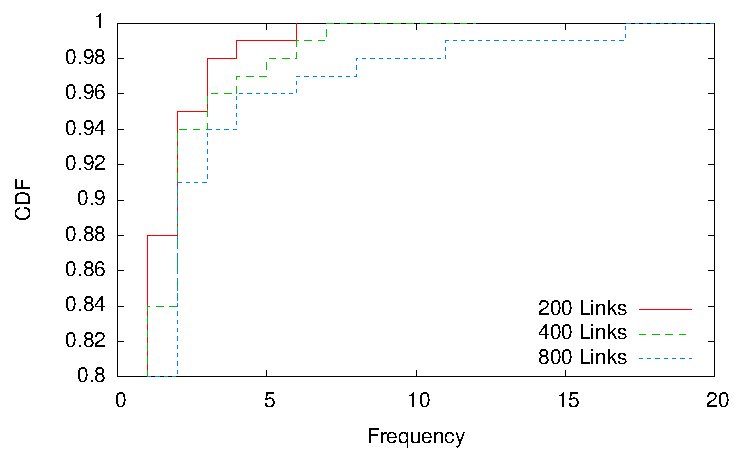
\includegraphics[width=0.5\columnwidth]{./graphs/arg-scg-cdfs}
        \label{fig:link-freq-a}
    }
    \subfloat[][Link Frequency (Normalised by from time)] {
        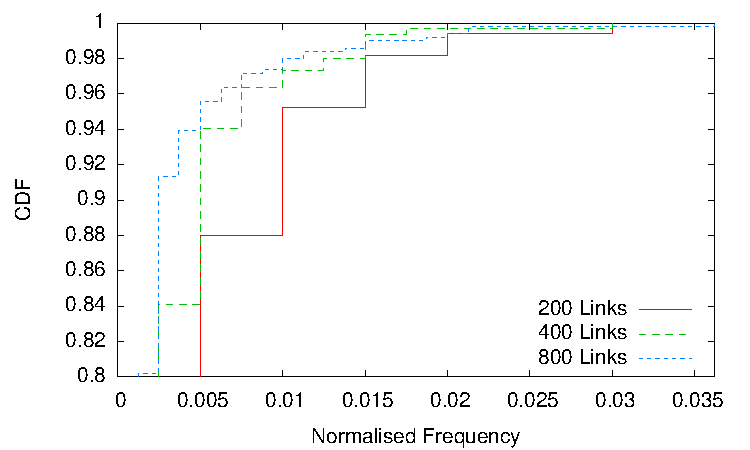
\includegraphics[width=0.5\columnwidth]{./graphs/arg-scg-cdfs-norm}
        \label{fig:link-freq-b}
    }

    \caption{CDFs of Argentina vs. Serbia and Montenegro link frequencies with varying numbers of links in the table}
    \label{fig:link-freq}
\end{figure}

The size of these tables may quickly be filled with requests with only a small frequency. \autoref{fig:link-freq-a} displays a CDF of link frequencies for one table with varying number of links in it. It can be seen that when there are 800 links, roughly 80\% of these have a frequency of one. These small frequencies may not be useful. Therefore, there are a few ways to reduce the size of the table. The first technique will reduce the resolution of the table by grouping similar times together. For example, in \autoref{tab:links}, the values 271 and 279 could be rounded down to a single value of 270. Then all matching values can be easily aggregated. This technique would most likely be used to at least round down to the nearest keyframe. As playback of media can only start from a keyframe, then it makes sense it always round the \emph{from} and \emph{to} times to the nearest preceding keyframe.

The second method aims to remove ``noise'' from the data. Each frequency can be transformed by some operations, such as a division or a right bit shift. Any frequencies which become zero or less would be removed from the table. Any values large enough to be significant will be kept, and the long tail of small results will be lost. A count of how often the table is reduced in this way must be kept to enable the table to be aggregated easily with other servers.

A final suggested technique would use the concept of aging, whereby entries in the table that have not be observed recently are removed from the table. This technique may provide the most relevant entries at the cost of additional overhead for each entry.

An evaluation of these techniques has not been conducted in a real system, and is therefore left for future work. However, the system has been designed to be lightweight and take advantage of how the delivery systems normally operate. The client, for example, only needs to send a small amount of additional information piggy-backed on existing communications. Additionally the servers do not have to handle any ``heavy'' per-client state, and instead only store the links table, which even if large would only consume 10-50~kilobytes\footnote{Based on 12~bytes per row, and between 800--4000 rows.} per media object.

%\todo{Put the results of these method here!!!!}

\section{Hybrid Delivery}

This section discusses how existing peer-to-peer (P2P) delivery techniques are unable to provide a sufficient level of interactivity to adequately support the workload analysed in this thesis. To improve the performance of P2P delivery, this section discusses a hybrid approach which can use the best features of two main classes of streaming P2P. These two classes are `pull' and `push', which have previously been described in \autoref{sect:peer-to-peer}.

To recap, push based systems configure the peers in a tree topology, and disseminate the content efficiently throughout the tree. This however does not give the peer freedom to seek within the stream, as everyone in the tree is at the same playback point. To seek, the peer would therefore need to join another tree, causing long seek delays.

The pull based system do not typically try to configure the peers into any structured way, instead creating random meshes of connections between the peers. Each peer must advertise the segments of the media they currently have stored locally. Peers may then request these segments arbitrarily, allowing them to play back the media in a sequential manner, or if they wish, seek to any segment and resume from there. This however requires a high amount of overhead as segment advertisements must be continually exchanged and each segment is only received after an solicited request.

The remainder of this section describes a hybrid approach which constructs the peers into multiple push-based trees using a periodic broadcast technique. The peers also form a light weight pull-based mesh, so they can use a P2P patching technique to allow for quick seeking. The following section describes these typically multicast/server orientated broadcasting and patching techniques, and how they relate to peer-to-peer. Following this, design, analysis and evaluation of the hybrid scheme is discussed.

\subsection{Periodic Broadcast and Patching}
    %Nic has read

    It is cheaper in terms of resources to serve ten users via a single multicast stream, then to serve the same ten users via unicast. Creating a single multicast channel decreases network load, as only $1/10$ of the bandwidth is needed, and also reduces requirements placed on the the server, such as the memory and disk IO bandwidth. However, it is not always possible to ensure that the users all wish to start watching at the same time; batching was therefore created to solve this~\cite{dan1994spf,aggarwal1994apb,viswanathan1996mav,hua1996sba}.

    Batching in its simplest form groups users with the same playback point together and delays them receiving the media until a suitable multicast stream can be found/created to accommodate the full group. This works well if the media is periodically broadcast~\cite{chiueh1995pba} on multiple multicast channels at fixed intervals apart. This technique is also called staggered broadcasting. When a client joins or seeks to a specific point~\cite{grant1994mpv}, they wait until one of the channel's playback points matches their required playback point. However, this causes a long delay, for example, if a 60~minute video is broadcasted over 10 evenly distributed channels, it can take at most 6 minutes to view any requested location, but on average only 3 minutes. To allay this issue, enhancements such as harmonic broadcasting~\cite{juhn97hbv} or patching can be employed.

    Patching (or sometimes called Stream Tapping~\cite{carter1997sta}) extends batching by adding a mechanism to remove the start-up delay whilst still utilising multiple dedicated channels~\cite{hua1998pam}. When a client requests a playback location which can not instantly be served by an existing channel, a separate patching channel is created. This can occur when the client first views the content, or if they seek to an arbitrary point. The client then requests both the patching channel and a dedicated channel whose playback point is later than the requested playback location. The patching channel contains the data required to catch up with the dedicated channel and is typically unicast from a content server or sometimes from neighbouring clients~\cite{kulkarni2008ast}. This then allows the client to begin playback instantly from the patching channel and buffer from the dedicated channel. Once the patching channel catches up with the client's buffer, the patching channel is stopped.

    The idea was extended to reduce the number of required dedicated channels. For example, consider there are two dedicate channels one being 10~minutes behind than the other. If a client is currently viewing the channel which is behind, they may start to patch from the ahead channel. After 10~minutes they would have caught up with the ahead channel and thus can disconnect from their behind channel. This then might allow the channel to be freed if no other users are viewing it.

    The duration for which the patching channel is used is called the \emph{patching window}~\cite{cai1999opp}. The size of the window can impact performance, for example, the \emph{greedy patching} scheme tries to minimise the number of multicast channels by allowing the patching window to be as long as the content's duration. It has been shown that being too greedy can result in less data sharing~\cite{hua1998pam}. The opposite of greedy patching is \emph{grace patching}, which schedules a new multicast channel when the client's buffer is smaller than the patching window.

%~\cite{gao1999siv}  eager2001mbr griwodz2000tlp
    A middle ground is controlled multicast, which adds access controls limiting how many patching channels can be created. For example, the controlled \emph{CIWP} algorithm~\cite{gao1999siv} uses a mathematically optimal scheduling algorithm that limits the rate at which patching channels are created. Another technique, Lambda Patching~\cite{griwodz2000tlp}, allows the server to decide on the patching window sizes, based on currently observed popularity and interarrival times.

    A final scheme is \emph{transition patching} which increases the size of the patch window, but allows multiple clients to share a patch stream, thus increasing bandwidth sharing~\cite{cai1999ebs}. The efficiency of these patching schemes has been measured~\cite{bradshaw2001pba, eager2001mbr}, modelled~\cite{tan2002qos} and optimised when considering factors such as video length, client buffer size and request rate~\cite{cai1999opp, eager1999oae, sen1999ops}.

    Although patching was originally designed to provide simple video-on-demand, it also enables interactivity. More recently, Ma~\emph{et~al.} optimised patching for high levels of interactivity~\cite{ma2005bep}. However their evaluation used non-realistic interactivity patterns. Rocha~\emph{et~al.} tested patching with more realistic interactive patterns and found that patching did not scale well under high levels of interactive requests. With low levels of interactivity, patching performed sufficiently. However, with medium to high interactivity, patching performed in a similar way to serving each client with an individual unicast stream~\cite{rocha2005sms}.

    %Piggybacking, speeds up one stream by a small amount, ie 10\% to allow it to catch up with another.

% Golubchik, L., J. Lui, and R. Muntz. Adaptive piggybacking: a novel technique for data sharing in video-on-demand storage servers. ACM Multimedia Systems Journal, 4(3): 140�155, 1996.
% P�ris, J.-F. An interactive broadcasting protocol for video-on-demand, Proceedings of the 20th International Performance of Computers and Communication Conference, pages 657�664, April 2001.

\subsection{Delivery Methods}

To compared a peer-to-peer hybrid approach to the existing push and pull methods, three delivery mechanisms are defined and evaluated. This section describes the three mechanisms in detail.

\subsubsection{Push -- Periodic Broadcast over TBCP}

The first of the three approaches aims to group similar users together on a multicast substrate. Given the lack of support for network multicast, we use an application-level multicast (ALM) algorithm, specifically the Tree Building Control Protocol~\cite{mathy01otb}, which in practice is a protocol to arrange the peers in a push-based P2P tree.

\emph{Periodic broadcast} can then be used in order to provide the illusion of true video-on-demand. Staggered broadcast is its simplest form, involving a number of multicast channels for a given video, and beginning each at an interval evenly distributed throughout its length~\cite{dau95cab}. Users may then move forwards and backwards throughout the stream by switching channels. The granularity of these operations is, however, limited by the interval between the available channels. Without allocating a large number of broadcast channels, startup/interaction latency may be unacceptable in longer pieces of media. An adaptation of this method is our push approach to delivering the media, in that content nodes broadcast the same segments of content to as many nodes as possible simultaneously, where TBCP trees are generated as required to act as periodic broadcast channels.

\subsubsection{Pull -- Peer-to-Peer}
\label{sect:pull}

The second delivery method considered, representative of the pull approach to delivery, is the use of a peer-to-peer, BitTorrent-like protocol. BitTorrent implements a tit-for-tit incentives mechanisms, to discourage free-riders\footnote{Peers who chose to not contribute to the network, thus obtaining a service at no cost to themselves.}. A beneficial side-effect of involving time-sensitive data in such a network is that the incentives that drive the system become more pronounced. In other words, due to the tit-for-tat exchange mechanism,  would be encouraged to contribute, as to improve the probability of receiving the segments they require in a timely fashion. Such protocols are not without drawbacks in the context of streaming media, however.

Firstly, the most common issue is that media playback requires sequential segments of a piece of content; BitTorrent instead delivers them effectively randomly. A solution often proposed to handle the need for sequential delivery is to apply a sliding-window to the data being distributed. Peers then have upper and lower boundaries for the segments which they are interested in downloading, and prioritise their requests accordingly.

Secondly, startup latency should be minimised; BitTorrent's reliance on other peers optimistically unchoking newcomers means this is not the case. Shar~\emph{et~al.} and Vlavianos~\emph{et~al.} amongst others have noted and responded to issues such as these~\cite{shar07ppm,vlavianos06beb}. A simple solution is to ensure that established peers perform optimistic unchoking on a more regular basis; Shah and P\^{a}ris show that, when combined with a sliding window approach, significant improvements over the base protocol can be achieved~\cite{shar07ppm}. We therefore employ similar methods to gain the same benefits.

\subsubsection{Hybrid -- Periodic Broadcast with P2P Patching}

Finally, the third method examined is a hybrid of both the push and pull methodologies. By using TBCP-based periodic broadcast trees in conjunction with peer-to-peer patching, clients can share data enabling them to reach the current broadcast point rapidly. To clarify, when a client joins a periodic broadcast channel, they do not need to wait for channel to reach the desired playback point, but can instead request segments from their neighbours as quickly as possible until the broadcast channel reaches the required position. This system is similar to the one described by Guo and Ammar~\cite{guo2004slv}. They used periodic broadcast over ALM, supported by server based patching. They showed promising results, however, their workload was an artificial start-to-finish.

\subsection{Experiment}

Three key variables to be considered for a delivery system are the size of the audience, the nature of the content (workload) and the network resources available. We also vary \emph{peer-to-peer usage}, in terms of the number of connections they are allowed to make to other peers. For example, if in an unrestricted environment there were 200 peers, a value of 10\% P2P usage would reduce the number returned to just 20. By varying this value, the effect of peer-to-peer patching on the hybrid method can be observed: at 0\% usage, the method is identical to the normal periodic broadcast over ALM, whereas at 100\% usage, the peer-to-peer scheme is made use of as much as possible. The increasing effect of the peer-to-peer patching system in the hybrid approach can therefore be observed in an incremental fashion relative to both the pure ALM and pure P2P delivery methods. Naturally, this does not affect the pure ALM approach, as no variance is seen in its results for plots of this type.

%\subsection{Workloads}

To obtain results that provide a comparison of how particular delivery schemes may handle different pieces of content, varied workloads are considered. These can be classified as follows:

\begin{description}
  \item[Start-to-Finish] Used for baseline comparison, where clients do not use any interactivity features. Media is viewed in a start-to-finish fashion, although the start and end points are not necessarily the same between clients.

  \item[Interactive] This workload is derived from the analysis and modelling conducted in \autoref{chap:evaluation}. In essence, the unique aspect of these workloads is large pieces of content with relatively short areas of high interest, highlighting how well a particular approach handles large differences in popularity between segments.
\end{description}

%\subsection{Metrics}

Beyond the workloads, the metrics used are selected to reflect both network provider and user satisfaction, based on resource usage efficiency and perceived quality of service respectively. The first metric considered, therefore, is \emph{network stress} in terms of the amount of data delivered on the network, normalised to the worst case in a given simulation.

The second metric used is `timely' segments, \emph{i.e}, one which arrived before its playback deadline. An \emph{average fraction of timely segments received per client} is therefore the average value, on a per-client basis, for the total number of timely segments divided by the total number of segments required by that client.

Finally, \emph{segment utility} is considered: the number of media segments actually used in playback in comparison with the total number sent over the network. Given that a client may receive segments superfluous to their requirements (\emph{e.g.}, buffering five minutes when the client only watches one. This metric provides a measure of network efficiency relative to the data that clients actually consume.

%\subsection{Overview}

A high-level overview of the experimental setup is as follows: 1,000 routers exist in a GT-ITM generated topology graph~\cite{gtitm}. The graph is of a realistic transit-stub configuration, wherein a single node exists per transit domain, but many exist per stub. Content node(s) (those sourcing the media) are attached to the aforementioned transit node(s), whereas clients are attached to randomly selected members of the stub domain(s). The content node(s) are connected via highly provisioned links, whereas, the clients are limited to a typical asymmetric link (1Mbit down, 256kb up).

The group size used in the simulations is 500 clients, and delivery of some subset of the piece of content per client is made using the appropriate method described for each simulation. Each client possesses an individual playback buffer, which should not underflow if user-satisfaction is to be achieved.

In our custom simulation environment, the overall delivery process is modelled in a number of steps over several iterations, whereas the content itself is handled as a series of sequential `segments'. Firstly, a realistic workload is generated (according to the models from \autoref{chap:evaluation}), wherein the clients are provided with individual lists of segments they will be required to obtain within the timeframe of the simulation.

Following workload generation, clients must interact with the delivery structures to begin the acquisition of segments. In the pull peer-to-peer approach, delivery proceeds as described in \autoref{sect:pull}. The push and hybrid approaches, however, primarily use TBCP periodic broadcast trees, meaning the initial step is for clients to determine which tree(s) will contain the segment(s) they require, and where they are rooted (\emph{i.e.}, the address to join). In the simulations this is achieved through a lookup process on a single node for simplicity, although in a real-world deployment with numerous videos of many segments each, a more sophisticated arrangement may be appropriate.

Following location of the correct tree for the required segment(s), a client must then wait on the periodic broadcast to roll-around to the required playback point for consumption. In the hybrid approach, the peer-to-peer mechanism can now be used to speed this process somewhat, by attempting to rapidly patch required segments that the client would otherwise have to wait for. Note that clients also have to use the knowledge of segment-tree mappings obtained from the lookup service to anticipate when trees must be switched, as to avoid suboptimal resource usage through nodes being present in a tree unnecessarily.

\subsection{Results}

\begin{figure}[t]
    \centering

    \subfloat[][Network cost of delivering] {
        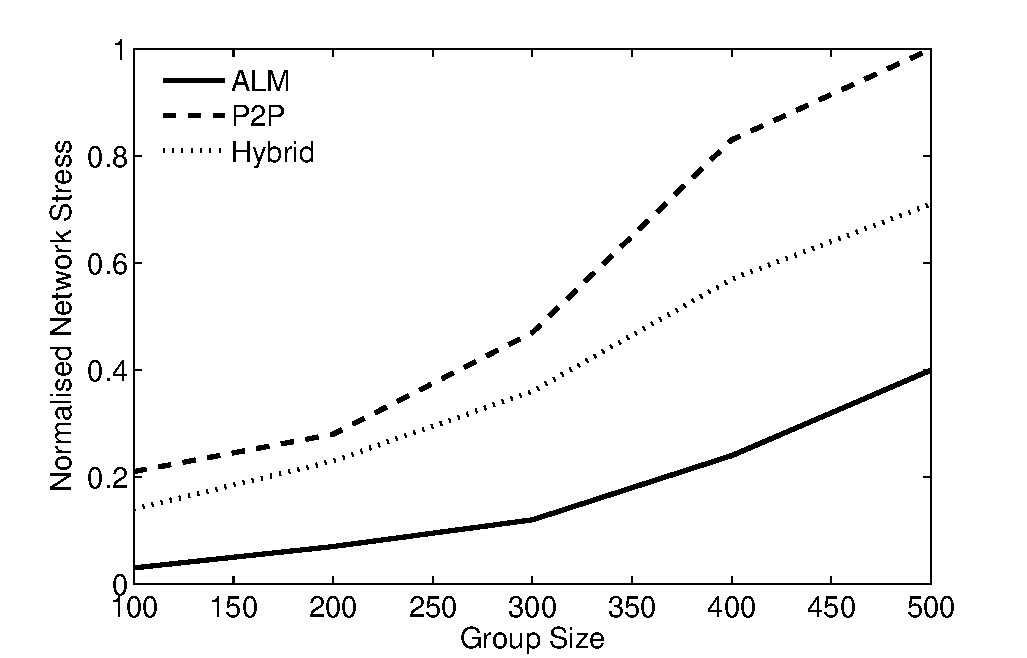
\includegraphics[width=0.5\columnwidth]{./graphs/netintsize}
        \label{fig:netintsize}
    }
    \subfloat[][User satisfaction during delivery] {
        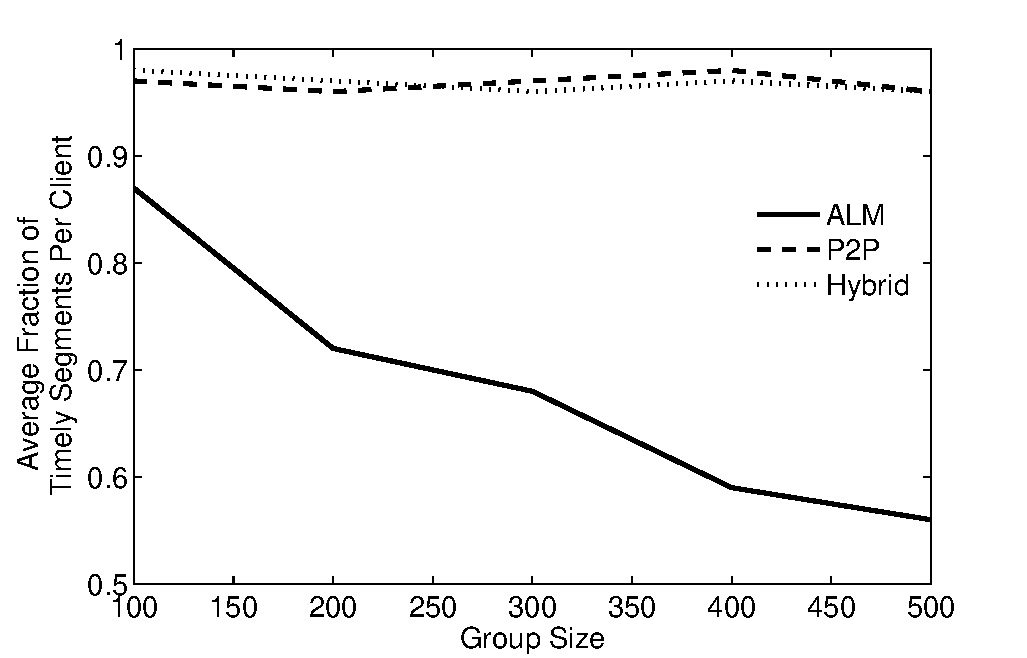
\includegraphics[width=0.5\columnwidth]{./graphs/userintsize}
        \label{fig:userintsize}
    }
    \caption{Delivering a Interactive workload with varied group size}
\end{figure}

\autoref{fig:netintsize} shows the resulting network cost across the delivery methods for an interactive workload with varying group sizes. The amount of traffic created for the ALM-based methods is shown to be lower than pull peer-to-peer; significantly so for large groups. A delivery method being low cost, however, is of little use unless it can deliver an equivalent quality of service. \autoref{fig:userintsize} shows that this is not the case for pure ALM, as an initially high level of timely segments reduces rapidly with increasing group size. Such a result may be indicative of this approach being unable to handle large, interactive groups well, possibly due to the joining overhead associated with switching between highly populated broadcast trees. Indeed, when delivering a `start-to-finish' workload (not shown), pure ALM was found to provide a level of performance similar to the other methods for the considered metrics.

\begin{figure}[t]
    \centering

    \subfloat[][Delivery of an interactive workload] {
        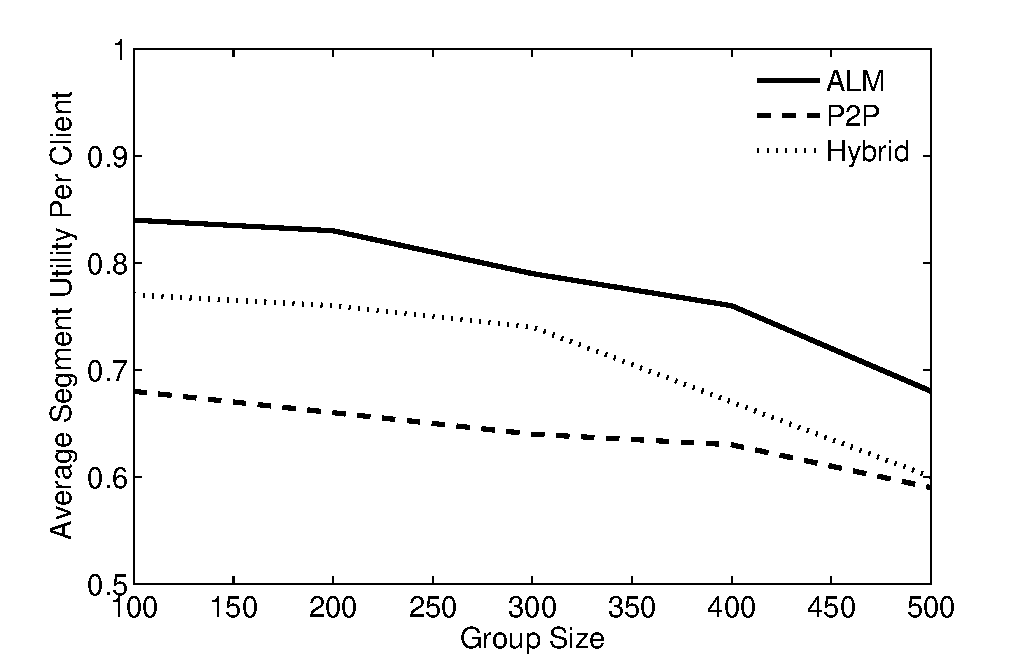
\includegraphics[width=0.5\columnwidth]{./graphs/utilintsize}
        \label{fig:utilintsize}
    }
    \subfloat[][Delivery of a start-to-finish workload] {
        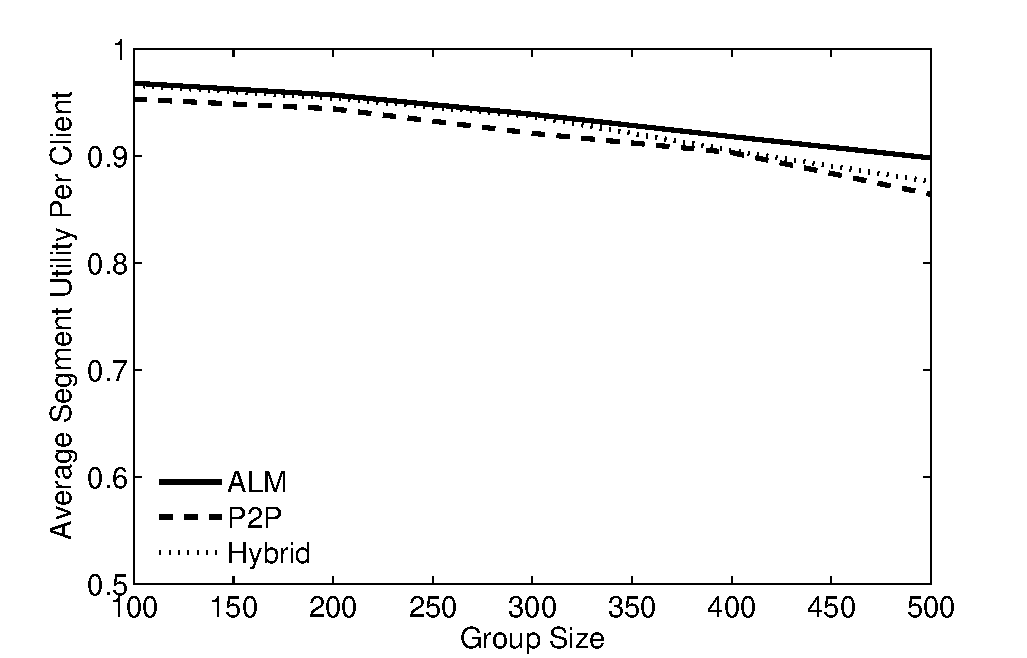
\includegraphics[width=0.5\columnwidth]{./graphs/utilstfsize}
        \label{fig:utilstfsize}
    }
    \caption{Overall segment utility during delivery with varied group size}
    \label{fig:util_size}
\end{figure}

% How can Pull/Hybrid have lower "segment utility" than push? Surely only the segments needed
% would actually be requested in pull. Perhaps they arrive late? But no, because that contradicts figure 5.7b
% Could have low utility of buffered, and this buffer was thrown away

\autoref{fig:util_size} show the average fraction of useful segments that were delivered during each simulation on a per client basis. Interestingly, \autoref{fig:utilintsize} indicates that for a high-interactivity workload, up to 40\% of segments on the network could be sent fruitlessly, with the factor of interactivity separating the delivery methods noticeably. In contrast, \autoref{fig:utilstfsize} shows that when the workload is start-to-finish, each of the schemes achieves a similar level of overall utility, working at an efficiency of around 85\% upwards at all times, with little to separate the methodologies. The `wasted' segments in these cases are most likely due to congestion, and accordingly show an increase with group size.

\subsubsection{Varying Peer-to-Peer Usage}

\begin{figure}[t]
    \centering

    \subfloat[][Delivery of an interactive workload] {
        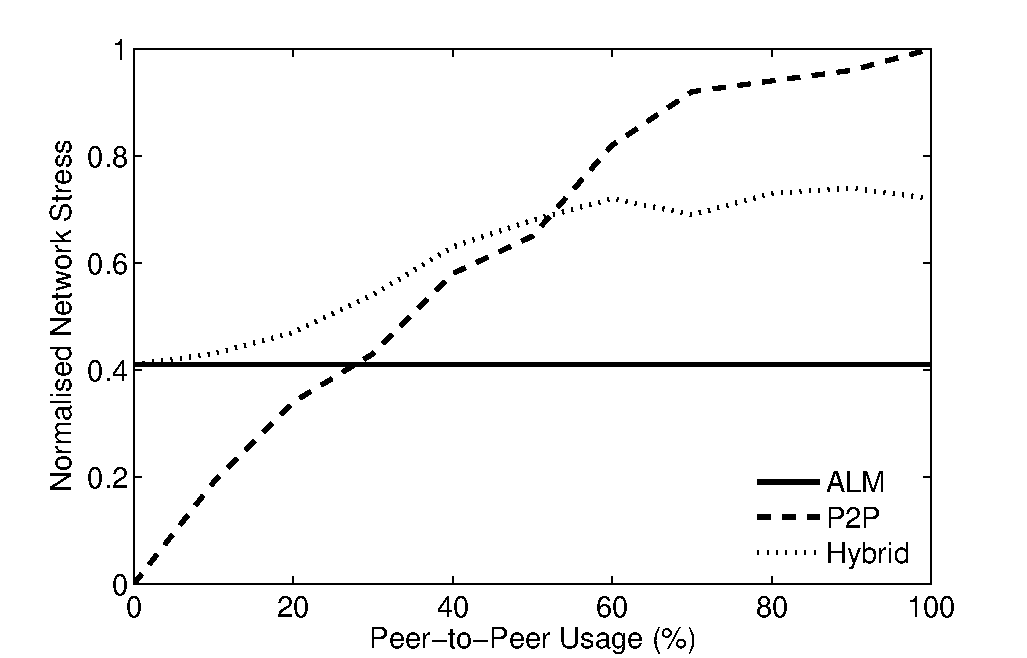
\includegraphics[width=0.5\columnwidth]{./graphs/netintpeer}
        \label{fig:netintpeer}
    }
    \subfloat[][Delivery of a start-to-finish workload] {
        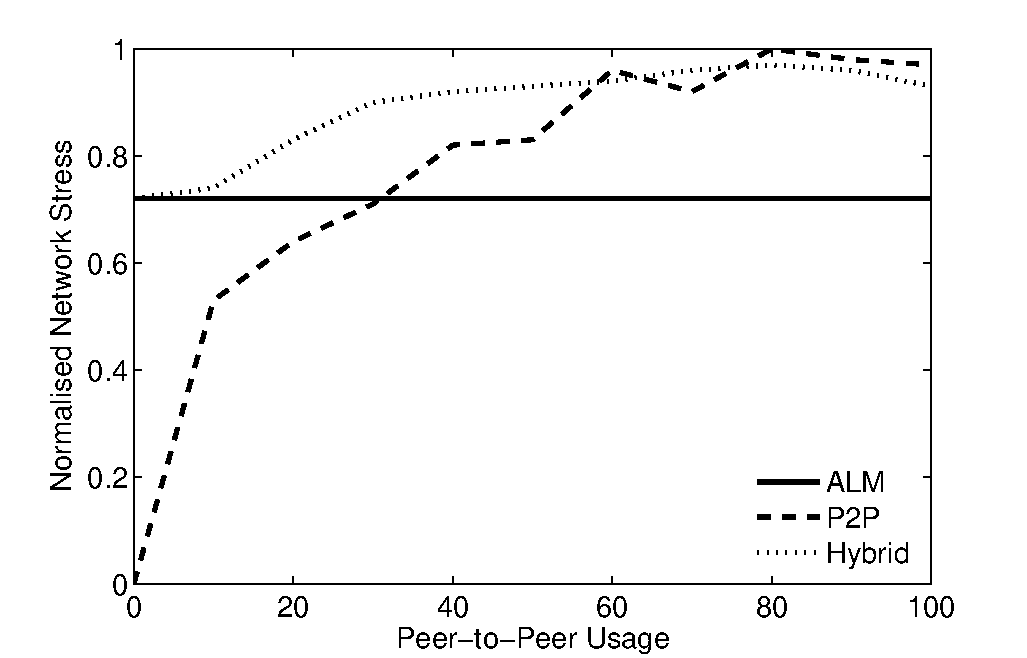
\includegraphics[width=0.5\columnwidth]{./graphs/netstfpeer}
        \label{fig:netstfpeer}
    }
    \caption{Network cost of delivery with varied peer-to-peer size}
\end{figure}

\begin{figure}[t]
    \centering

    \subfloat[][Delivery of an interactive workload] {
        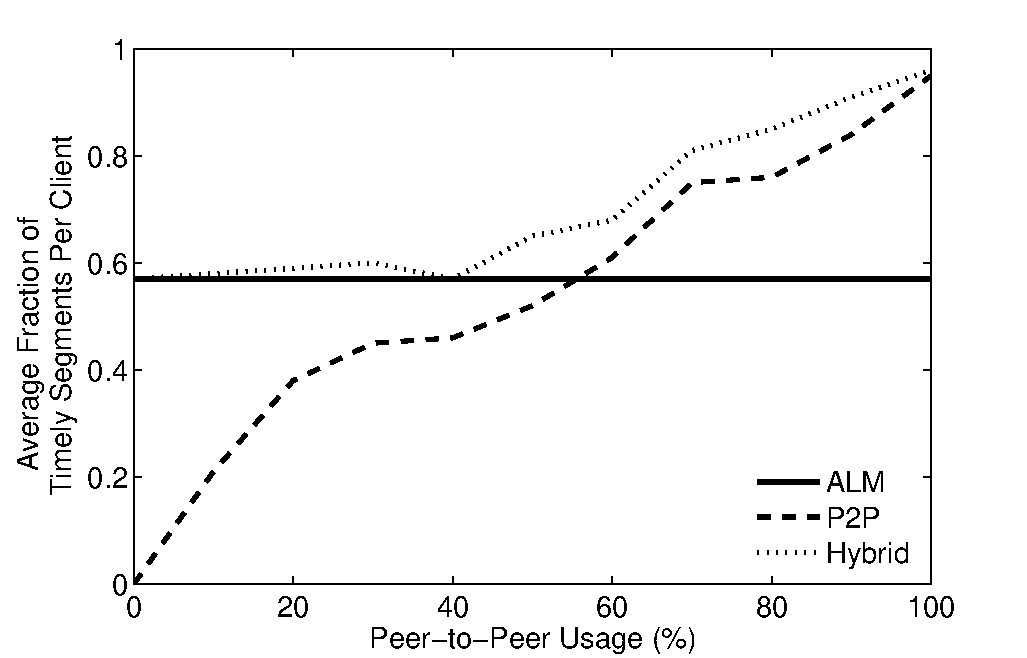
\includegraphics[width=0.5\columnwidth]{./graphs/userintpeer}
        \label{fig:userintpeer}
    }
    \subfloat[][Delivery of a start-to-finish workload] {
        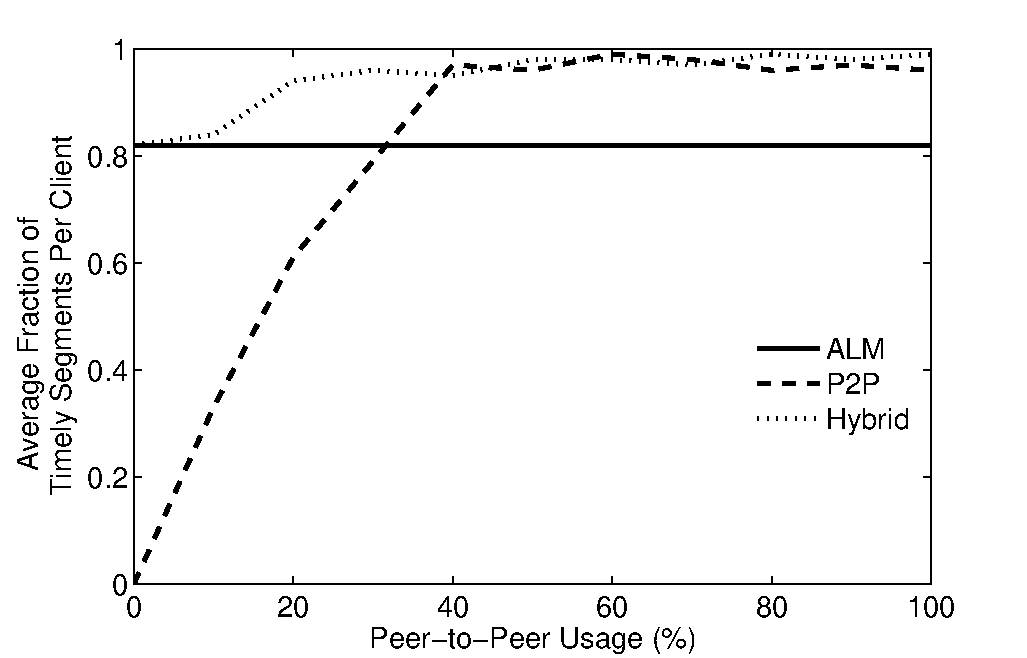
\includegraphics[width=0.5\columnwidth]{./graphs/userstfpeer}
        \label{fig:userstfpeer}
    }
    \caption{User satisfaction during delivery with varied peer-to-peer size}
\end{figure}

\autoref{fig:netintpeer} shows the network stress in terms of data delivered per link for an interactive workload, normalised to the `worst case' of full peer-to-peer usage. As simulations run to the point where clients no longer have any interest in receiving segments, the reduced traffic in the low usage scenarios for the peer-to-peer case is to be expected. Two notable points on this plot are around 25\% and 50\% peer-to-peer usage, where the pull method crosses over the ALM and hybrid approaches respectively. Following the latter intersection, the hybrid method appears to level off while pull P2P continues to increase. Dependent on the user satisfaction for these schemes at these points, this indicates that the hybrid method can produce a consistently lower amount of network traffic relative to push P2P, although the addition of patching is resulting in twice the amount produced by ALM alone. A key point to consider regarding the high network cost of pull P2P is that the ALM-based approach is exploiting the concept of locality in building shortest-path trees to the highly provisioned content nodes. In the pull peer-to-peer case, this does not happen, and many segments are likely being sent lengthy distances between groups of clients viewing the same section of video, potentially across multiple network transit/stub domains.

If the first figures are considered as showing network cost, then the likes of \autoref{fig:userintpeer} show the resultant level of `user satisfaction', in terms of the average fraction of timely segments per client. Recall that two particular points of interest in \autoref{fig:netintpeer} were around the 25\% and 50\% peer-to-peer usage marks. In this figure, however, no significant improvement over pure ALM is shown until around the latter of these points: the 50\--60\% mark. It therefore seems that without the ability to disseminate a large amount of P2P data, the use of the pull P2P approach just results in additional overhead for this type of workload. As the usage increases beyond this point, however, the number of timely segments being delivered increases significantly for both the schemes that make use of P2P. In almost all cases, however, the hybrid method outperforms pull P2P, although not by a large amount. This may be due to the sequential nature of the media playback -- when periodic broadcast is used, most of the data that clients need will be pushed to them anyway -- the pull approach may only be particularly useful when clients have to seek to new points in the media. The high level of interactivity in the workload used for this particular figure may therefore explain the relatively poor performance of pure ALM.

\autoref{fig:netstfpeer} shows the result of a simulation similar to that conducted for \autoref{fig:netintpeer}, but with users consuming the content `start-to-finish'. The network cost is found to be closer between the three methods in this case than with a high-interactivity workload, supporting the idea that user interactivity can be more costly for certain delivery methods. Interestingly, when examined in conjunction with \autoref{fig:userintpeer}, it can be observed that the pull P2P approach outperforms the hybrid method under these metrics when ``peer-to-peer usage'' is around the 40\% mark. This particular simulation result may therefore run contrary to the initial expectation that periodic broadcast may be better suited than pull P2P for many users viewing the media in a generally sequential fashion. Also note, however, that the average fraction of timely segments for pure periodic broadcast in this low-interactivity scenario is significantly better; effectively double that of the high-interactivity workload, and more akin to the results obtained for the high-interactivity workload with small group sizes. This result is as expected, as reduced interactivity correspondingly results in fewer clients jumping between broadcast trees, fewer setup delays, and thus fewer untimely segments according to the clients' demands.

\subsubsection{Additional Nodes}

\begin{figure}[t]
    \centering

    \subfloat[][Additional shared-content] {
        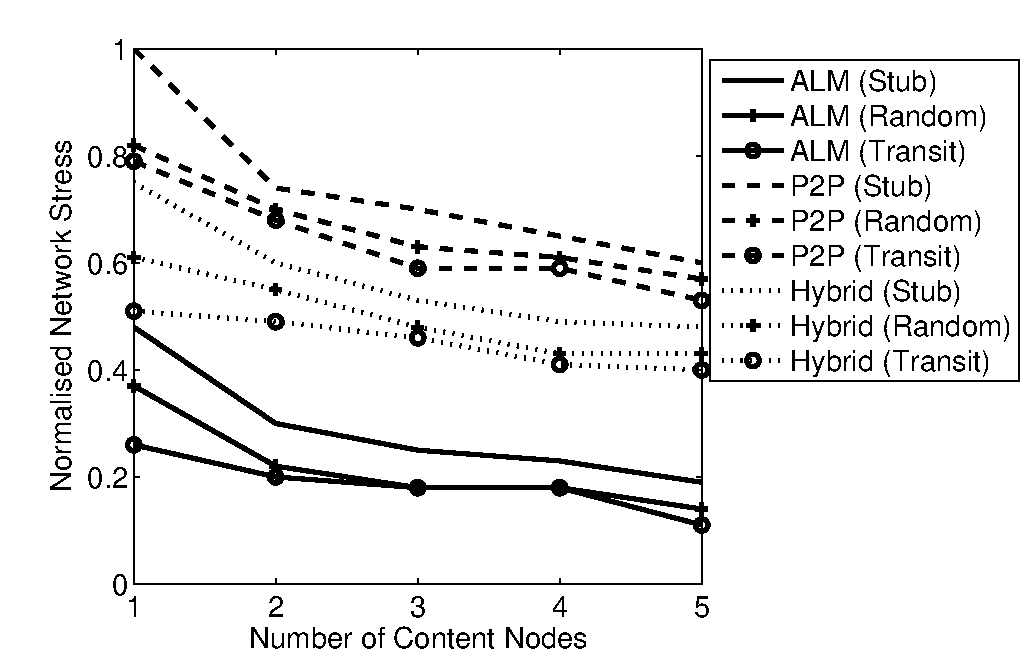
\includegraphics[width=0.5\columnwidth]{./graphs/nodeshared}
        \label{fig:nodeshared}
    }
    \subfloat[][Additional redundant-content nodes] {
        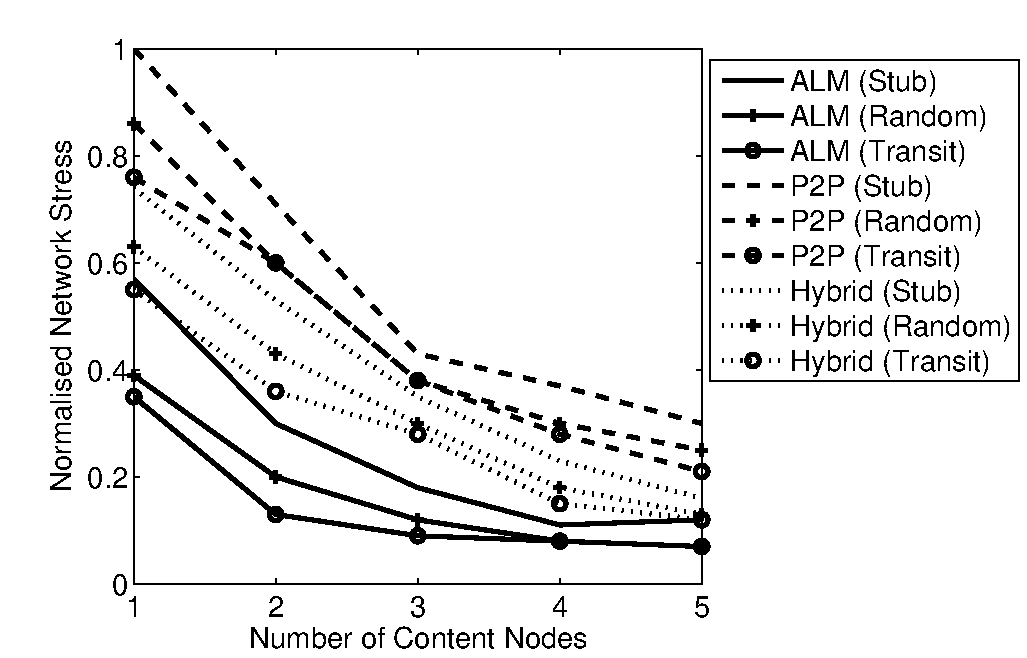
\includegraphics[width=0.5\columnwidth]{./graphs/noderedundant}
        \label{fig:noderedundant}
    }
    \caption{Effect of additional nodes on overall network stress}
\end{figure}

In all cases, as shown in \autoref{fig:nodeshared} and \autoref{fig:noderedundant}, the addition of extra resources in the form of additional content sources (\emph{i.e.}, the roots of trees or seeds in swarms) is beneficial, with similar trends observed regardless of the delivery method being used. This is especially true of the case when content is made available in a redundant fashion rather than simply being `striped' across nodes. The exact placement of these nodes also has some impact, albeit a less significant one, with a slightly diminishing effect as more nodes are made available.

\subsubsection{Key Observations}

From these findings, several points become clear. Regarding network costs in terms of traffic generated, pull P2P is relatively expensive in comparison with the simpler ALM approach. This cost is offset, however, by a resilience to large group sizes and high levels of interactivity in comparison with ALM. Fortunately, when the methods are combined into the hybrid method, network cost is lower than the pull peer-to-peer case, albeit higher than ALM alone, making it an effective compromise. In all cases, larger group sizes result in an increase in the amount of network traffic, and this also has a slightly negative effect on segment utility.

In terms of user satisfaction, larger groups have little effect on the fraction of timely segments received when the peer-to-peer system is involved under any level of interactivity. This is also largely true for the case of pure ALM when low levels of user interactivity are observed, but when users begin to jump around within a video, ALM performs significantly worse. This effect can be attributed to the lengthy join delays when the broadcast trees are particularly long, coupled with the standard waiting period on the broadcast channel to receive the segment(s) the user requires. Naturally, this does not affect the pull approach of the peer-to-peer method, and when this is combined with the ALM scheme, the peer-to-peer system acts as a means of patching; providing the media segments required in an on-demand fashion until the push scheme has stabilised. For similar reasons, segment utility is quite similar across all methods for low interactivity workloads, but when high levels of interactivity occur, there is a marked difference between the schemes. For instance, while the peer-to-peer approach typically achieves high-levels of user satisfaction, a larger percentage of segments are wasted relative to ALM. The naturally sequential nature of the broadcast over ALM may therefore be acting in its favour here, given that users are highly likely to want large numbers of media segments delivered in this fashion.

\subsection{Conclusion}

From the results observed, we can conclude that while peer-to-peer methodologies are certainly feasible for the delivery of interactive content from the user perspective, they are somewhat network-intensive. In contrast, a more traditional approach based around classical periodic broadcast techniques over an application-level multicast structure apparently work well for smaller numbers of passive viewers, but encounters problems when user interactivity and group size increase. The combination of these two approaches, broadly pull and push, can, however, offer a good compromise that provides adaptability to varying conditions in terms of audience size, interactivity levels, and the resources available. Across all the delivery methods considered, providing additional resources in terms of extra content nodes is beneficial, with their placement relative to clients being increasingly important dependent on their abundance.

It is therefore apparent that mixing a live distribution approach such as application-level multicast with an appropriate peer-to-peer patching mechanism over a typical network infrastructure (\emph{i.e.}, typically lacking in IP multicast support) can provide a workable solution for delivery of on-demand video with interactivity support in a CDN environment. Given the wide variety of possible workloads, delivery methods and variables, much potential exists for future work in this field.
